%% IMPLEMENTATION

\section{Language Choice}
Java was the language used in implementing the applications outlined in the
previous chapters. Android applications can be created using Java, C or C++.
Since each application running on an Android device is executed in a Java
Virtual Machine (JVM), Java is the primary development language used on the
platform.\\
C or C++ could also be used thanks to the Android NDK, but as the official
documentation suggests\footnote{NDK documentation - http://goo.gl/OykZpe},
should only be used for very specific, CPU-intensive tasks and one should not
use the NDK because they prefer writing applications in C/C++.

In addition to these lower-level languages, many other languages can be used
thanks to third-party transpilers such as PhoneGap (JavaScript), Apportable
(Objective-C/Swift), Titanium (JavaScript) etc.\\
These tools allow developers to write code in different languages and either
run them in a \texttt{WebView} using JavaScript and HTML5 or transpiles the
source code into Java and compiles as if the developer had used Java in the
first place.

\section{Development Tools}

\subsection{IDE}
When it comes to Android Development, two main IDEs stand out:
\begin{enumerate}
\item Eclipse\\
    Eclipse was the original official Android development environment and is
    still used by many developers. It uses a plugin called ADT
    (Android Development Tools) to interact with ADB and manages SDKs etc.
\item Android Studio\\
    Android Studio is currently the official IDE for Android and comes with
    many improvements over Eclipse. It is built on top of the popular IntelliJ
    IDE, and is tailored specifically for Android development. This allows it
    to have specific Android tools and functionality 'baked in', thus not
    requiring any plugins to begin development.\\
    Android Studio also comes with built-in functionality for the Gradle build
    system, allowing for easier dependency management and a more sophisticated
    build environment.
\end{enumerate}

With Android's new Gradle build system, it is possible to use no more than a
text editor and the Android build tools from the command line to compile and
run an application. However, for building interfaces and the editing tools
an IDE can offer, Android Studio was used.

\subsection{Version Control}
Android Studio has built-in support for the most popular version control
systems. Git was chosen due to the sheer volume of libraries available on Github
and Google's sample projects from the Android documentation site also use it.

%% Communication

\section{Android Wear Communication}

This section details how an Android device communicates with its Android Wear
counterpart using Bluetooth and the Android Wear APIs. Communication was a
fundamental part of the project and is used to send messages, commands or entire
objects from handheld to smartwatch and vice-versa.

\subsection{Pre-requisites}
In order for a smartwatch application to communicate with its counterpart
handheld application, a few conditions must be met.

\begin{enumerate}
\item Android Wear Companion App\\
    As mentioned in previous chapters, the official Android Wear Companion App
    must be installed, and the wearable must connected and paired with the
    handheld through this app.
\item Package name
    Both the wearable and the handheld applications must use the same package
    name in their \texttt{AndroidManifest.xml} files. The APIs will not work
    correctly and communication will not occur between the applications if one
    of the package names is different.
\end{enumerate}

\subsection{Communication Types}
With Android Wear there are two main types of communication:
\begin{enumerate}
\item Messages\\
    Messages are blobs of data limited in size to 100KB, which are sent from one
    device to another. The destination of the message must be known when
    sending.\\
    Messages are useful for RPC or a client-server messaging protocol.
\item DataItems
    DataItems are blobs of data which when created are automatically synced
    across the Android Wear network and replicated on all connected nodes.
    DataItems are useful for ensuring data is kept the same on both handheld and
    wearable.
\end{enumerate}

All communication is handled by the system. The API for doing this is all dealt
with by the \texttt{GoogleApiClient}. This API client connects to Google Play
Services and allows for interaction with Google services, such as Android Wear,
Play Games, Google Drive etc.\\
As a result, multiple APIs can be accessed via a single
\texttt{GoogleApiClient}, however, Google recommend using a single
\texttt{GoogleApiClient} instance for dealing solely with Android Wear
communications. This prevents failure callbacks for users that don't have a
wearable device if they are trying to access another service.

\begin{lstlisting}[language=Java]
GoogleApiClient mGoogleApiClient = new GoogleApiClient.Builder()
        .addApi(Wearable.API)
        .addConnectionCallbacks(mConnectionCallbacks)
        .addOnConnectionFailedListener(
            mOnConnectionFailedListener)
        .build();
\end{lstlisting}

Here we create a GoogleApiClient and tell it which API to connect to, which in
this case is the Wearable API. We also set its connection callbacks and
listeners.
This allows us to get notified of connection events such as when the device is
connected, suspended etc.

\texttt{mConnectionCallbacks} and \texttt{mOnConnectionFailedListener} might
look something like the following:

\begin{lstlisting}[language=Java]
mConnectionCallbacks = new ConnectionCallbacks() {
    @Override
    public void onConnected(Bundle connectionHint) {

        // device has been connected succefully to the
        // Wearable/Handheld

    }

    @Override
    public void onConnectionSuspended(int cause) {

        // the connection has been suspended. Device out
        // of range, or unavailable

    }
}

mOnConnectionFailedListener =
        new OnConnectionFailedListener() {
    @Override
    public void onConnectionFailed(ConnectionResult result) {
        
        // the connection failed to initialize

    }
}

\end{lstlisting}

In order to use the \texttt{GoogleApiClient}, it must be connected to Google
Services. Here is how we achieve this with the Android Activity lifecycle:

\begin{lstlisting}

public class MyActivity extends Activity {

    ...

    @Override
    public void onResume() {
        super.onResume();
        mGoogleApiClient.connect();
    }

    @Override
    public void onPause() {
        super.onPause();
        mGoogleApiClient.disconnect();
    }

    ...

}

\end{lstlisting}


% MESSAGE APPI
\subsection{Message API}

Once the \texttt{GoogleApiClient} is connected, it can be used to send messages
and/or \texttt{DataItem}s. In order to send a message we need the following
information:

\begin{enumerate}
\item A connected \texttt{GoogleApiClient}.
\item A \texttt{Node} to send the message to.
\item A path for the message so the receiving application can decide which
    action to apply.
\item A payload
\end{enumerate}

All paths on Android Wear communications are relative to a base URI which Wear
uses to communicate. These URIs are of the form:
\texttt{wear://<node-id>/<path>}

\begin{lstlisting}[language=Java]
Wearable.MessageApi.sendMessage(
        mGoogleApiClient,
        nodeId,         // String : the id of the receiving Node
        "/start/music", // String : the path of the message

        // byte[] : the payload of the message
        "song-123".getBytes()
);
\end{lstlisting}

On the receiving end, when a message is received, we can check whether it's the
message we are interested in by checking the path:

\begin{lstlisting}[language=Java]
...
if (path.equals("/start/music") {
    // open music player
}
\end{lstlisting}

Using this technique we can send multiple different messages and perform
different actions on the handheld based on the path of the messages.

\subsubsection{Receiving Messages}
Sending messages from the handheld to the watch or vice-versa is only useful if
the other side is listening for these messages. In order to perform actions or
respond received messages, the device must register itself with the Android Wear
API and implement a callback method for when a message is received.\\
In order to start receiving messages from the counter-part application, the
application must register itself as a listener to the \texttt{MessageApi}:

\begin{lstlisting}[language=Java]

@Override
public void onResume() {
    super.onResume();
    // add the listener
    Wearable.MessageApi.addListener(mGoogleApiClient, mListener);
}

...

@Override
public void onPause() {
    super.onPause();
    // remove the listener
    Wearable.MessageApi.removeListener(mGoogleApiClient, mListener);
}
\end{lstlisting}

The listener for receiving message events looks like this:

\begin{lstlisting}[language=Java]
@Override
public void onMessageReceived(MessageEvent messageEvent) {

    // get the path of this message's URI
    String path = messageEvent.getPath();

    // perform an action based on the path
    if (path.equals("/start/music")) {
        // start the music application
        Intent intent = new Intent(this, MusicActivity.class);
        startActivity(intent);
    }

}
\end{lstlisting}

Using this send-respond architecture, a client-server model can be created
whereby the wearable can request data from the handheld using a custom
protocol, and the handheld can reply with the requested data.\\
It also enables using the wearable as a remote to start activities or trigger
actions on the handlheld, such as launching a compose new email activity or
starting/stopping music playback.

%% DATA API
\subsection{Data API}
Previously we discussed sending messages and performing actions upon receiving
them. Android Wear provides another form of communication allowing developers
to synchronize data across both the handheld and wearable. Whenever the data is
updated on one size, an event is triggered on the other notifying it of the
change.

This is useful for sending images, or keeping data consistent across both
devices. For example, the handheld could retrieve contact data from it's
database using SQLite and store it in the wearable \texttt{DataApi}. Provided
the wearable has registered itself for receiving data changes, the data would
then present itself to the wearable where it could be displayed or stored in
it's own SQLite database.

\subsubsection{Inserting DataItems to the Data Layer}
In order to insert something into the data layer, we must first create a
\texttt{PutDataRequest} which is very similar to a java \texttt{Map} but that
deals with byte arrays. To make things simpler, we can use a
\texttt{PutDataMapRequest}, which behaves more like a traditional \texttt{Map}
where we can store key-value pairs of primitive types.

As with all communication on Android Wear, we must also specify a path for this
data's URI. We can then hand this \texttt{PutDataMapRequest} off to the system
for synchronization.

\begin{lstlisting}[language=Java]
// create the PutDataMapRequest with a given path
PutDataMapRequest putDataMapRequest =
        PutDataMapRequest.create("/settings");

// get a more traditional map from the PutDataMapRequest
DataMap dataMap = putDataMapRequest.getDataMap();

// fill the map with some primitive data
dataMap.putString("color", "#FFAAFF");
dataMap.putFloat("rating", 4.5f);
dataMap.putInt("refresh_interval", 20);

// convert our traditional map back to a byte[] map
PutDataRequest putDataRequest = putDataMapRequest
        .asPutDataRequest();

// hand the request off to the system to put the map
// in the data layer
Wearable.DataApi.putDataItem(mGoogleApiClient, dataMap);
\end{lstlisting}

In the code above, we created a map containing some basic settings and put the
map into the data layer. This means the data will be accessible from either
device. If the handheld or wearable are not connected or out of range, the
system will queue the request and perform when possible. This does not have to
be handled by the developer.

\subsubsection{Retrieving DataItems from the Data Layer}
Retrieving \texttt{DataItem}s from the data layer is slightly different. If we
know the path of the data we want to retrieve, we can use

\begin{lstlisting}[language=Java]
Wearable.DataApi.getDataItem(mGoogleApiClient, uri);
\end{lstlisting}

where \texttt{uri} is the \texttt{URI} of the item we want to retrieve. This
involves building the URI manually which can be cumbersome and erroneous. A
simpler way of retrieving \texttt{DataItem}s is by fetching all items and
filtering them by path as shown below.

\begin{lstlisting}[language=Java]
DataItemBuffer dataItemBuffer = Wearable.DataApi
        .getDataItems(mGoogleApiClient)
        .await();

for (DataItem dataItem : dataItemBuffer) {
    String path = dataItem.getUri().getPath();

    // check we are using the correct 
    if (path.equals("/settings")) {
        // create a DataMapItem from the given DataItem
        // so we can access our map
        DataMapItem dataMapItem = DataMapItem
                .fromDataItem(item);
        DataMap dataMap = dataMapItem.getDataMap();

        // get the settings back out of the map
        String color = dataMap.getString("color");
        Float rating = dataMap.getFloat("rating");
        int refreshInterval= dataMap.getInt("refresh_interval");
    } else if (path.equals("/other-data")) {
        ...
    }
}

// make sure to release the buffer to prevent leaking memory
dataItemBuffer.release();
\end{lstlisting}

%% Data layer events

\subsubsection{Data Layer Events}

In order to be able to synchronize data across the handheld and wearable
devices, listeners must be created and added to the \texttt{DataApi}. Then, 
whenever \texttt{putDataItem()} is called, the listeners on both sides of the
communications will be notified.

For example, when the wearable application first starts, it may call
\texttt{getDataItems()} to get all the \texttt{DataItem}s currently stored in
the data layer and store the relevant information in memory. It might then add
a listener to the \texttt{DataApi} in order to watch changes to this data and
update its internal data structures for that data.

\begin{lstlisting}[language=Java]

@Override
public void onResume() {
    super.onResume();
    Wearable.DataApi.addListener( mGoogleApiClient,
            mListener);
}

@Override
public void onPause() {
    super.onPause();
    Wearable.DataApi.removeListener( mGoogleApiClient,
            mListener);
}

\end{lstlisting}

The above code demonstrates how to add a listener for data layer events to an
\texttt{Activity}. When the \texttt{Activity} is suspended to the background
we genereally don't want to interact with the events. A \texttt{Service} can be
used to interact with data layer events when the application is not in the
foreground. This will be explained in the next section.\\
Below is what \texttt{mListener} might look like for handling data layer events

\begin{lstlisting}[language=Java]

mListener = new DataApi.DataListener() {

    @Override
    public void onDataChanged(DataEventBuffer dataEventBuffer) {
        
        // there may be multiple events handled at once
        for (DataEvent dataEvent : dataEventBuffer) {

            // get the DataItem from the event
            DataItem dataItem = dataEvent.getDataItem();
            String path = dataItem.getUri().getPath();

            // ignore items that we are not interested in
            if (! path.equals("/settings") {
                continue;
            }

            // we only want to perform actions on data that
            // has changed
            if (event.getType() == DataEvent.TYPE_CHANGED) {
                DataMap dataMap = DataMapItem
                        .fromDataItem(dataItem)
                        .getDataMap();

                // get the new settings from the map
                String newColor = dataMap.getString("color");
                Float newRating = dataMap.getFloat("rating");
                int newRefresh = dataMap
                        .getInt("refresh_interval");
            }
        }

    }

};

\end{lstlisting}

%% WearableListenerService

\subsection{WearableListenerService}

In this section communicating with wearables from a \texttt{Service} will be
discussed. Android Wear APIs come with a special \texttt{Service} designed
specifically for communicating with wearables:
\texttt{WearableListenerService}.

In order to use \texttt{WearableListenerService}, it must be extended by a
custom \texttt{Service}. Just like any regular Android \texttt{Service}, it must
first be declared in the \texttt{AndroidManifest.xml} file but with a special
\texttt{intent-filter}:

\begin{lstlisting}[language=XML]

<service android:name=".DataLayerListenerService">
    <intent-filter>
        <action android:name=
            "com.google.android.gms.wearable.BIND_LISTENER" />
    </intent-filter>
</service>

\end{lstlisting}

Unlike a normal Android \texttt{Service}, it must not be started or stopped.
The system handles this.\\
This \texttt{Service} must extend \texttt{WearableListenerService} and
override it's communication methods. In order to listen for communication
events, a \texttt{GoogleApiClient} must be created and the listeners must be
attached as described in previous sections.

\begin{lstlisting}[language=Java]

public class DataLayerListenerService extends
        WearableListenerService {
    
    @Override
    public void onCreate() {
        super.onCreate();

        mGoogleApiClient = new GoogleApiClient.Builder()
                ...
                .build();

        // since we are running in a Service, we can call
        // a blocking method. Calling this on the main thread
        // of an Activity would cause an error and the async
        // mGoogleApiClient.connect() would have to be used
        // instead
        mGoogleApiClient.blockingConnect();

        // attach the listeners
        Wearable.MessageApi.addListener(mGoogleApiClient, this);
        Wearable.DataApi.addListener(mGoogleApiClient, this);

    }

    @Override
    public void onDestroy() {
        super.onDestroy();

        // remove the listeners
        Wearable.MessageApi.removeListener(mGoogleApiClient, this);
        Wearable.DataApi.removeListener(mGoogleApiClient, this);

        // ensure we disconnect from the Wearable API
        mGoogleApiClient.disconnect();
    }

    @Override
    public void onPeerConnected(Node peer) {
        super.onPeerConnected(peer);

        // called when the wearable and handheld have been
        // connected
    }

    @Override
    public void onDataChanged(DataEventBuffer dataEvents) {
        // code to deal with changed or delete data events
    }

    @Override
    public void onMessageReceived(MessageEvent messageEvent) {
        // code to run when message received
    }

}

\end{lstlisting}

This type of \texttt{Service} allows us to listen for communication events even
when the application is not in the foreground. This is quite a common case as
it is quite rare that a user would have the application open on both the
wearable and the handheld at the same time. In the Student Application discussed
in this report, a \texttt{WearableListenerService} is created on handheld and
acts as a server to the wearable. The \texttt{Service} could just as easily have
been created on the wearable, or on both.


%% ASSETS

\subsection{Syncing Assets}
Up to this point, syncing data and sending messages have been limited to 100KB
in payload. In order to send data of larger size such as images or audio files,
\texttt{Asset}s must be used. \texttt{Asset}s are attached to
\texttt{DataItem}s and are stored and retrieved in a similar way to any other
data stored in a \texttt{DataItem}.

\begin{lstlisting}[language=Java]

// get the Bitmap to send from the device's resources
Bitmap bitmap = BitmapFactory.decodeResource(
        getResources(), R.drawable.ic_launcher);

// here we need to convert the Bitmap into an Asset
// an Asset can be created from a byte array, so we must
// get the byte array from the Bitmap
ByteArrayOutputStream byteStream =
        new ByteArrayOutputStream();
bitmap.compress(Bitmap.CompressFormat.PNG, 100, byteStream);
Asset asset = Asset.createFromBytes(byteStream.toByteArray());


// here we create a PutDataMapRequest just like we did
// for putting primitive values into the data layer
PutDataMapRequest putDataMapRequest =
        PutDataMapRequest.create("/image");

// get the DataMap for this PutDataMapRequest
DataMap dataMap = putDataMapRequest.getDataMap();

// add the Asset to the DataMap
dataMap.putAsset("icon", asset);

// sync the DataMap containing the Asset into the data layer
Wearable.DataApi.putDataItem(mGoogleApiClient,
        dataMap.asPutDataRequest());

\end{lstlisting}

In order to receive the Asset on the other side of the communication, we must
implement the \texttt{DataApi.DataListener} and check for the event in
\texttt{onDataChanged()}.

\begin{lstlisting}[language=Java]

...

@Override
public void onDataChanged(DataEventBuffer dataEvents) {

    for (DataEvent dataEvent : dataEvents) {
        DataItem dataItem = dataEvent.getDataItem();
        String path = dataItem.getUri().getPath();

        if (path.equals("/image")) {
            DataMap dataMap = DataMapItem
                    .fromDataItem(dataItem)
                    .getDataMap();

            // retrieve the Asset from the DataMap
            Asset asset = dataMap.getAsset("icon");
            onAssetReceived(asset);

        }
    }

}

private void onAssetReceived(Asset asset) {

    // Assets have unique file descriptors on the device
    // get the file descriptor for the given Asset
    // this method is called asynchronously, to get an
    // immediate repsonse, await() could be used, but only
    // in a background thread
    Wearable.DataApi.getFdForAsset(mGoogleApiClient, asset)
            .setResultCallback(new
                ResultCallback<DataApi.GetFdForAssetResult>()
                    {

        @Override
        public void onResult(DataApi.GetFdForAssetResult
                getFdForAssetResult) {

            // re-construct the Bitmap from the file
            InputStream assetInputStream =
                    getFdForAssetResult.getInputStream();
            Bitmap mapBitmap = BitmapFactory
                        .decodeStream(assetInputStream);

            // do something with the received Bitmap

        }

    });
}

...

\end{lstlisting}


%% SERIALIZATION

\subsection{Object Serialization}

When communicating between handheld and wearable, a common use case might
require a Java object to be used on both devices, for example a calendar event.
In order to achieve this, the object must be broken down into it's primitive
data, transfered as an array of bytes and reconstructed on the other side of
the connection. Android has built-in interfaces for this, namely the
\texttt{Parcelable} interface.

When an object implements \texttt{Parcelable} it describes itself in terms of
it's primitive data such as \texttt{Integer}s, \texttt{Float}s and
\texttt{String}s. This data can then be written to a \texttt{Parcel} object and
"marshalled" into a byte array. \texttt{Parcelable} objects can be nested within
other \texttt{Parcelable} objects. The \texttt{Parcelable.Creator<T>} interface
specifies how an object of type \texttt{T} should be recreated from a
\texttt{Parcel}.

For Android Wear, \texttt{DataMap}s could also be used instead of
\texttt{Parcel}s, but since \texttt{Parcel}s are used frequently in Android
development, such as passing an object between Activities, \texttt{Parcel}s
may be more versatile for re-use.

Below is an example of a simple object which implements \texttt{Parcelable}

\begin{lstlisting}[language=Java]

public class CalendarEvent implements Parcelable {

    private String title;
    private int numAttendees;
    private Date date;

    // nested Parcelable oject
    private Parcelable myObject;

    ...

    // Describe the kinds of special objects contained in
    // this Parcelable's marshalled representation
    @Override
    public int describeContents() {
        return 0;
    }

    @Override
    public void writeToParcel(Parcel out, int flags) {
        out.writeString(title);
        out.writeInt(numAttendees);
        out.writeLong(date.getTime());
        out.writeParcelable(myObject);
    }

    // the object that will handle reconstructing the event
    public static final Creator<CalendarEvent> CREATOR =
            new Creator<CalendarEvent>() {

        @Override
        public CalendarEvent createFromParcel(Parcel source) {
            // reconstruct the CalendarEvent from the given
            // Parcel
            CalendarEvent event = new CalendarEvent();
            event.setTitle(source.readString());
            event.setNumAttendees(source.readInt());
            event.setDate(new Date(source.readLong()));

            // reconstruct the nested Parcelable object
            event.setMyObject(source.readParcelable(
                MyObject.class.getClassLoader()));
            return event;
        }

        @Override
        public CalendarEvent[] newArray(int size) {
            // create a new CalendarEvent array
            return new CalendarEvent[size];
        }

    };

}

\end{lstlisting}

Now when an instance of the \texttt{CalendarEvent} class is created, it can
be put into a parcel and marshalled as follows:

\begin{lstlisting}[language=Java]

// get a free Parcel instance
Parcel parcel = Parcel.obtain();
CalendarEvent event = new CalendarEvent();

// write the event into the Parcel using the methods
// implemented above
event.writeToParcel(parcel, 0);

// set the data pointer back to the start ready for reading
parcel.setDataPosition(0);

// to then be able to transfer the Parcel with Android Wear
DataMap dataMap = ...
String key = "cal-event";
dataMap.putByteArray(key, parcel.marshall());

// the DataMap can then be synced using the data api or
// message apis

// recycle the Parcel when it is no longer needed
parcel.recycle();

\end{lstlisting}

In order to read the serialized \texttt{Parcel} on the other side of the
connection, a \texttt{Parcel} must be obtained, and it must unmarshall the byte
array from the \texttt{DataMap}. Using the \texttt{CREATOR} instance created
above, the \texttt{CalendarEvent} can be reconstructed from the \texttt{Parcel}.

\begin{lstlisting}[language=Java]

DataMap dataMap = ... // get the DataMap from Android Wear

byte[] byteArray = dataMap.getByteArray(key);

Parcel parcel = Parcel.obtain();

// unmarshall the byte array into the new Parcel
parcel.unmarshall(byteArray, 0, byteArray.length);

// reset the data pointer to the start for reading
parcel.setDataPosition(0);

// read the parcel data, and create a CalendarEvent
CalendarEvent event = creator.createFromParcel(parcel);

parcel.recycle();

\end{lstlisting}

Of course if the code permits, a \texttt{DataMap} could be used directly instead
of a \texttt{Parcel}, but using a \texttt{Parcel} may allow the developer to
serialize the object for saving to disk or passing the object between processes
or activities.


%% Communication Threads
\subsection{Communication Threads}

The Android Wear communication APIs described in previous sections are all
carried asynchronously with callback methods called in background threads.
The APIs return a \texttt{PendingResult<T>} instance with the relevant
results from the API call.

Android does not allow updating of the user interface from a thread other than
the main UI thread. In order to update the UI on a result from an Android Wear
API call, a \texttt{Handler} must be used to post the UI code to the main UI
thread for execution. This can be done as follows:

\begin{lstlisting}[language=Java]

PendingResult<MessageApi.SendMessageResult> result;
result = Wearable.MessageApi.sendMessage(
        mGoogleApiClient, nodeId, path, messageBytes);

result.setResultCallback(new ResultCallback
        <MessageApi.SendMessageResult>() {
    @Override
    public void onResult(MessageApi.SendMessageResult result) {
        // called on a background thread when the message
        // has been sent
        onMessageResult(result);
    }
});

private void onMessageResult(final String result) {

    // perform non-UI logic here
    doSomething();

    // perform UI logic here
    (new Handler(Looper.getMainLooper())).post(new Runnable() {
        @Override
        public void run() {
            mTextView.setText("Result: "
                + result.getStatus().toString());
        }
    });

}

\end{lstlisting}

In order to run the UI logic on the main thread, a \texttt{Runnable} is posted
to the main \texttt{Handler} and gets scheduled for processing.

If an Android Wear comunications API method is called from a thread that is
already running in the background, there is no need to use callbacks at all.
\texttt{PendingResult}s have an \texttt{await()} method which blocks execution
until the result is ready for processing. If multiple API calls need to be made
in immediate succession, it might make sense to run them all on a background
thread and just use one callback for the overall result. This can be achieved
using an \texttt{AsyncTask}. The \texttt{await()} method cannot be run on the
main thread, if it is, the application will crash and throw an exception.

\begin{lstlisting}[language=Java]

(new AsyncTask<Void, Void, Void>() {
    
    @Override
    protected Void doInBackground(Void... params) {
        // make API calls
        MessageApi.SendMessageResult result;
        result = Wearable.MessageApi.sendMessage(
            mGoogleApiClient, nodeId, path, messageBytes).await();
        if (result.getStatus().isSuccess() {
            // make another API call
        }
    }

    @Override
    protected void onPostExecute(Void aVoid) {
        // execute callback method here
        // this method runs on the UI thread
    }

}).execute();

\end{lstlisting}


%% SENSORS

\section{Sensors}

Sensors allow devices to read data from the outside world. Applications can use
sensor data to monitor real-time data and perform actions on it, or present it
to the user in a more digestible way.

Android supports measuring raw data from many different types of sensors. The
availability of sensors depends on the device and version of Android it is
running. Android Wear is no different. Android Wear allows for the same APIs
to be used in detecting and measuring data from built-in sensors.

Android Wear provides the user with access to sensors a regular Android device
might not have access to. This project was carried out and tested on a
Samsung Gear Live device. On this device, there is a heart-rate monitor which
can measure the rate at which the heart beats by using a bright LED on the back
of the watch to illuminate the top of your wrist and measure the rate of the
pulsing of the blood.\\
This method requires the wearer to be completely still and that the LED be
completely clean to give an accurate reading. Even when these conditions are
met, there is still a certain skepticism as to how accurate this type of
monitor really is.

In any case, Android Wear provides the same APIs for accessing sensors on a
wearable as those used to achieve the same on a handset. The
\texttt{SensorManager} is used to query the availability of different
\texttt{Sensor}s at runtime. A \texttt{Sensor} object then provides methods
allowing you to discover the capabilities and retrieve information regarding
the underlying sensor such as resolution, maximum range.\\
The \texttt{SensorManager} also allows us to attach listeners to each sensor
to listen for events related to the sensor, such as when the accuracy of the
sensor changes or when the values of the sensor are updated or changed by the
underlying hardware for the sensor.

The below code listing demonstrates how one might sense heart-rate data from
a wearable device. The code could also be run on a handset device with no
errors, but would not return any data unless it was equipped with a heart-rate
monitor.

\begin{lstlisting}[language=Java]

public class HeartRateActivity extends Activity
        implements SensorEventListener {

    // the SensorManager is used to retrieve the heart-rate
    // sensor
    private SensorManager mSensorManager;

    // this is the heart-rate sensor itself which will be
    // used to measure the raw data
    private Sensor mHeartSensor;

    @Override
    public void onCreate(Bundle savedInstanceState) {
        super.onCreate(savedInstanceState);
        
        mSensorManager = (SensorManager)
                getSystemService(SENSOR_SERVICE);

        // ask the SensorManager for a heart-rate sensor
        // if there is no heart rate sensor present, this
        // will return null
        mHeartSensor = mSensorManager
                .getDefaultSensor(Sensor.TYPE_HEART_RATE);

    }

    @Override
    public void onResume() {
        // start listening for events on the heart sensor
        mSensorManager.registerListener(this, mHeartSensor,
                SensorManager.SENSOR_DELAY_NORMAL);
    }

    @Override
    public void onPause() {
        mSensorManager.unregisterListener(this,
            mHeartSensor);
    }



    @Override
    public final void onAccuracyChanged(Sensor sensor,
            int accuracy) {
        // called when the accuracy of the sensor has changed
    }

    @Override
    public final void onSensorChanged(
            SensorEvent event) {
        // event.values can be more than one
        // eg. accelerometer returns 3 values
        float heartRate = event.values[0];

        Log.d("HeartRateActivity", String.format(
            "Received heart rate %.0f", heartRate));
    }

}

\end{lstlisting}

\begin{figure}
    \centering
    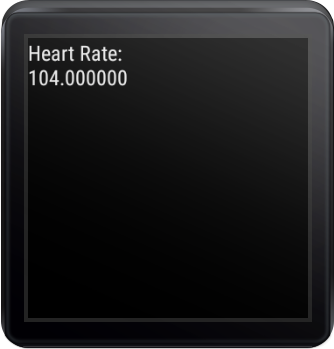
\includegraphics[width=0.4\textwidth]{heart-rate-monitor-activity.png}
    \caption{Activity monitoring heart-rate}
    \label{fig:awesome_image}
\end{figure}

If a higher degree of accuracy is needed, a higher sample rate can be specified
for measuring the raw sensor data. It should be noted however, that selecting a
higher sampling rate can consume more power than a slower sampling rate. As a
result it is recommended to use a high sampling rate only when necessary.\\
In the above example the default sampling rate of
\texttt{SensorManager.SENSOR\_DELAY\_NORMAL} was used. The available sampling
rates are listed below:
\begin{enumerate}
\item SENSOR\_DELAY\_NORMAL (default) - 200ms
\item SENSOR\_DELAY\_UI - 60ms
\item SENSOR\_DELAY\_GAME - 20ms
\item SENSOR\_DELAY\_FASTEST 0ms
\end{enumerate}

When attempting to listen on a sensor that is not available, the system should
continue running. When an application requires the use of a specific sensor,
that is to say the application needs it to function, it should declare so in
it's \texttt{AndroidManifest.xml} file. eg.

\begin{lstlisting}[language=XML]

<uses-feature
    android:name="android.hardware.sensor.accelerometer"
    android:required="true" />

\end{lstlisting}

Note that this is not necessary, but would help filter capable devices on the 
Google Play Store if submitted.
